\documentclass[12pt, notitlepage]{article}
%\usepackage[backend=biber]{biblatex}
\usepackage{amsmath}
\usepackage{listings}
\usepackage{graphicx}
\usepackage{caption}
%\usepackage{subcaption}
\usepackage{commath}
\usepackage{hyperref}
\usepackage{url}
\usepackage{xcolor}
\usepackage{textcomp}
\usepackage{dirtytalk}
\usepackage{listings}
\usepackage{wasysym}
\usepackage{float}
\usepackage{listings}
\usepackage[linesnumbered,lined,boxed,commentsnumbered]{algorithm2e}
\usepackage{subfig}

% Packages from derivations_fullproblem.tex
\usepackage[squaren]{SIunits}
\usepackage{a4wide}
\usepackage{array}
\usepackage{cancel}
\usepackage{amsmath}
\usepackage{amsfonts}
\usepackage{amssymb}
\usepackage{graphicx}
\usepackage{enumerate}
\usepackage{titling}

% Parameters for displaying code.
\lstset{language=python}
\lstset{basicstyle=\ttfamily\small}
\lstset{frame=single}
\lstset{keywordstyle=\color{red}\bfseries}
\lstset{commentstyle=\itshape\color{blue}}
\lstset{showspaces=false}
\lstset{showstringspaces=false}
\lstset{showtabs=false}
\lstset{breaklines}

% Define new commands
\newcommand{\expect}[1]{\langle #1 \rangle}
% Add bibliography
\begin{document}


\title{FYS-STK4155 - Project 2}
\author{Geir Tore Ulvik, Idun Kløvstad}
\begin{titlingpage}
\maketitle
\begin{abstract}
In this work four methods to sample or manipulate input data to learning
algorithms are explored: Random over-sampling, SMOTE, ADASYN, and balanced
weighting.
Several way to measure classifier performance are used, and the performance 
of logistic regression and a random forest classifier is evaluated based 
on how they perform on a binary classification problem. 
The data set chosen is payment data from an important bank in Taiwan,
where the data describes credit card holders, and the goal is predicting
whether a customer will default the next payment or not. 
The results presented show that logistic regression can classify the credit 
card data perfectly by applying a balanced weighting of the inputs. 
Random forests reached an accuracy of ~$95\%$ (cross-validation score). 
A possible explanation for the success of weighting the inputs compared 
to the other sampling methods is that some features in the data set may be 
far more crucial in determining the class than others, 
and weighting is the most efficient way of emphasizing these features through 
the learning process. Random forests do not gain similar improvement with
the same weighting, showing most improvement when using random over-sampling.
\end{abstract}
\end{titlingpage}
\section{Introduction}
Code, data and figures are available at the following GitHub address:
\href{https://github.com/geirtul/fys-stk4155/tree/master/project3}{GitHub repository}\\

In this project, we explore different ways to improve results of two binary
classifiers without hyperparameter tuning - Logistic regression and
Random forests. The methods used are of the over-sampling type and are as
follows: Random over-sampling, SMOTE, ADASYN, and balanced weighting of
inputs.

The data set chosen as input, is payment data The data set chosen is payment
data from an important bank in Taiwan, where the data describes credit card 
holders, and the goal is predicting whether a customer will default the 
next payment or not.

The same data set is used in an article from 2009 ~\cite{ComparisonData} 







\section{Theory}

%Consider putting in: general on ML 

%Consider adding theory from project1? 
%Until then: 
As the theory behond the three regression methods used as well as error 
estimates and the bootstrap method is covered in the previous 
project, we will not restate it here.

\subsection{The Ising model}\label{seq:isingtheory}
The ising model is a simple binary value system where the variables
in the model can take only two values. For examle \(\pm 1\) or \(0\) and \(1\). 
~\cite{Project2} 

We will look at the physicist's approach, and call the variables for spin.
~\cite{Project2}

Given an ensamble of random spin configurations we can assign an energy to
each state, using the 1D Ising model with nearest-neighbor interactions: 

\begin{equation}
	E = -J\sum\limits_{j=1}^N S_jS_{j+1} 
\end{equation}
J is the nearest-neighbor spin interaction, and \(S_j \epsilon {\pm 1}\) is a 
spin variable. N is the chain length. 
~\cite{HighBias}~\cite{Project2} 

In one dimension, this model has no phase transitions at finite temperature.
~\cite{Project2} 

To get a spin model with pairwise interactions between every pair of variables,
we choose the following model class: 

\begin{equation}
	E_{model}[S^i] = -\sum\limits_{j=1}^N\sum\limits_{k=1}^N J_{j,k} S_j^iS_{k}^i
\end{equation}
~\cite{HighBias} 

In this equation \(i\) represents a particular spin configuration. ~\cite{Project2}

The goal with this model is to determine the interaction matrix \(J_{j,k}\). 
As the model is linear in \(\mathbf{J}\), it is possible to use
linear regression.  

The problem can be recast on the form

\begin{equation}
	E_{model}^i = \mathbf{x}^i \cdot \mathbf{J}  
\end{equation}

\subsection{Logistic regression and classification problems}
Differently to linear regression, classification problems 
are concerned with outcomes taking the form of discrete variables. 
For a specific physical problem, we'd like to identify its state, say whether
it is an ordered of disordered system. ~\cite{LectureNotes-FysStk}

Logistic regression can be used to define the phases of the Ising
model.~\cite{LectureNotes} 

Configurations representing states below the critical temperature are called
ordered states, while those above the critical temperature are called 
disorderes states. ~\cite{Project2} 

The theoretical critical temperature for a phase transition is 
\(T_C \approx 2.269\). 

\subsection{Cost functions} 
In order for a network and a logistic regressor to improve it needs a way to 
track how it's performing. This is the purpose of a cost function. Essentially,
the cost function says something about how wrong the model is in classifying the
input. The objective in machine learning, and logistic regression, is then to minimize
this error.

The cost function used in this project is called the \textbf{cross-entropy}, or the
'negative log likelihood', and takes the form
\begin{equation}\label{eq:cross-entropy}
	\mathcal{C}(\hat{\beta})=-\sum_{i=1}^n  \left(y_i(\beta_0+\beta_1x_i) -\log{(1+\exp{(\beta_0+\beta_1x_i)})}\right)
\end{equation}

\subsection{Gradient Descent}
Minimizing the cost function is done using Gradient Descent.
The jist of it is that in order to optimize the weights or coefficients, and biases
to minimize the cost function, one can change their values to 

\begin{equation}\label{eq:delta-c}
	\frac{\partial \mathcal{C}(\hat{\beta})}{\partial \hat{\beta}} = -\hat{X}^T\left(\hat{y}-\hat{p}\right)
\end{equation}

\subsection{Accuracy score}
To measure the accuracy of the network, an accuracy score is defined as:
\begin{equation*}
	\text{Accuracy} = \frac{\sum_{i=1}^{n} I(t_i = y_i)}{n}
\end{equation*}
which is simply the number of correctly labeled states divided by the
total number of states. In the equation above, $I$ is the indicator function,
1 if $t_i = y_i$ and 0 otherwise. $t_i$ is the known correct label and $y_i$ is the
label output by the network.






%\section{Method}

\subsection{Producing data and recast problem}
To generate the training data, we used the code given in 
project2. 
The code a system with size \(L=40\) and \(1000\) different 
ising states and returns the Ising-energies. 

Then the problem was recasted as a linear regression model, using 
the regression methods from project1. The theory behind 
the Ising model and the recasting is described in ~\ref{seq:isingtheory}.

\subsection{Estimating the coupling constant of the one-dimensional Ising model using linear regression}

\subsection{Determining the phase of the 2D Ising model}
To determine the phase of the two dimensional Ising model we use 
logistic regression. Information about logistic regression can be found 
in section \ref{seq:logistic}. 

Out logistic regression method uses a cost function 
and gradient decent, which you can read about 
in sections ~\ref{seq:cost} and ~\ref{seq:gradient}.

We chose to use a stocastic gradient decent method. 

We use the data sets generated by Mehta et al ~\cite{HighBias}
and a fixed lattice of L x L = 40 x 40 spins in two dimensions.

To evaluate the model, we have used the accuracy score described in 
section ~\ref{seq:accuracy}. 

\subsection{Classifying with Neural Network}
The codebase provided in (cite neural network lecture notes) was
used as a base. However, the network was implemented using the sigmoid
activation function in the output layer as well, making the network
'tailored' to binary classification (only one output node). 
(Further Improvements in conclusion, softmax and layer spec)
The following code snippet is the bread and butter of the neural
network. Weights are initialized to random values following a
normal distribution (\lstinline{numpy.random.randn}), and biases
to the low value of $0.01$.
(Replace lstlistings with filenames and line-numbers.)
\begin{lstlisting}
def train(self):
    indices = np.arange(self.n_inputs)

    for i in range(self.epochs):
	for j in range(self.n_iter):
	    chosen_indices = np.random.choice(
		indices, size=self.batch_size, replace=False)

	    # Batch training data and targets
	    self.x_batch = self.x[chosen_indices]
	    self.y_batch = self.y[chosen_indices]

	    activations = self.feed_forward(self.x_batch)
	    self.backwards_propagation(activations)
\end{lstlisting}

\section{Results}
\begin{figure}[H]
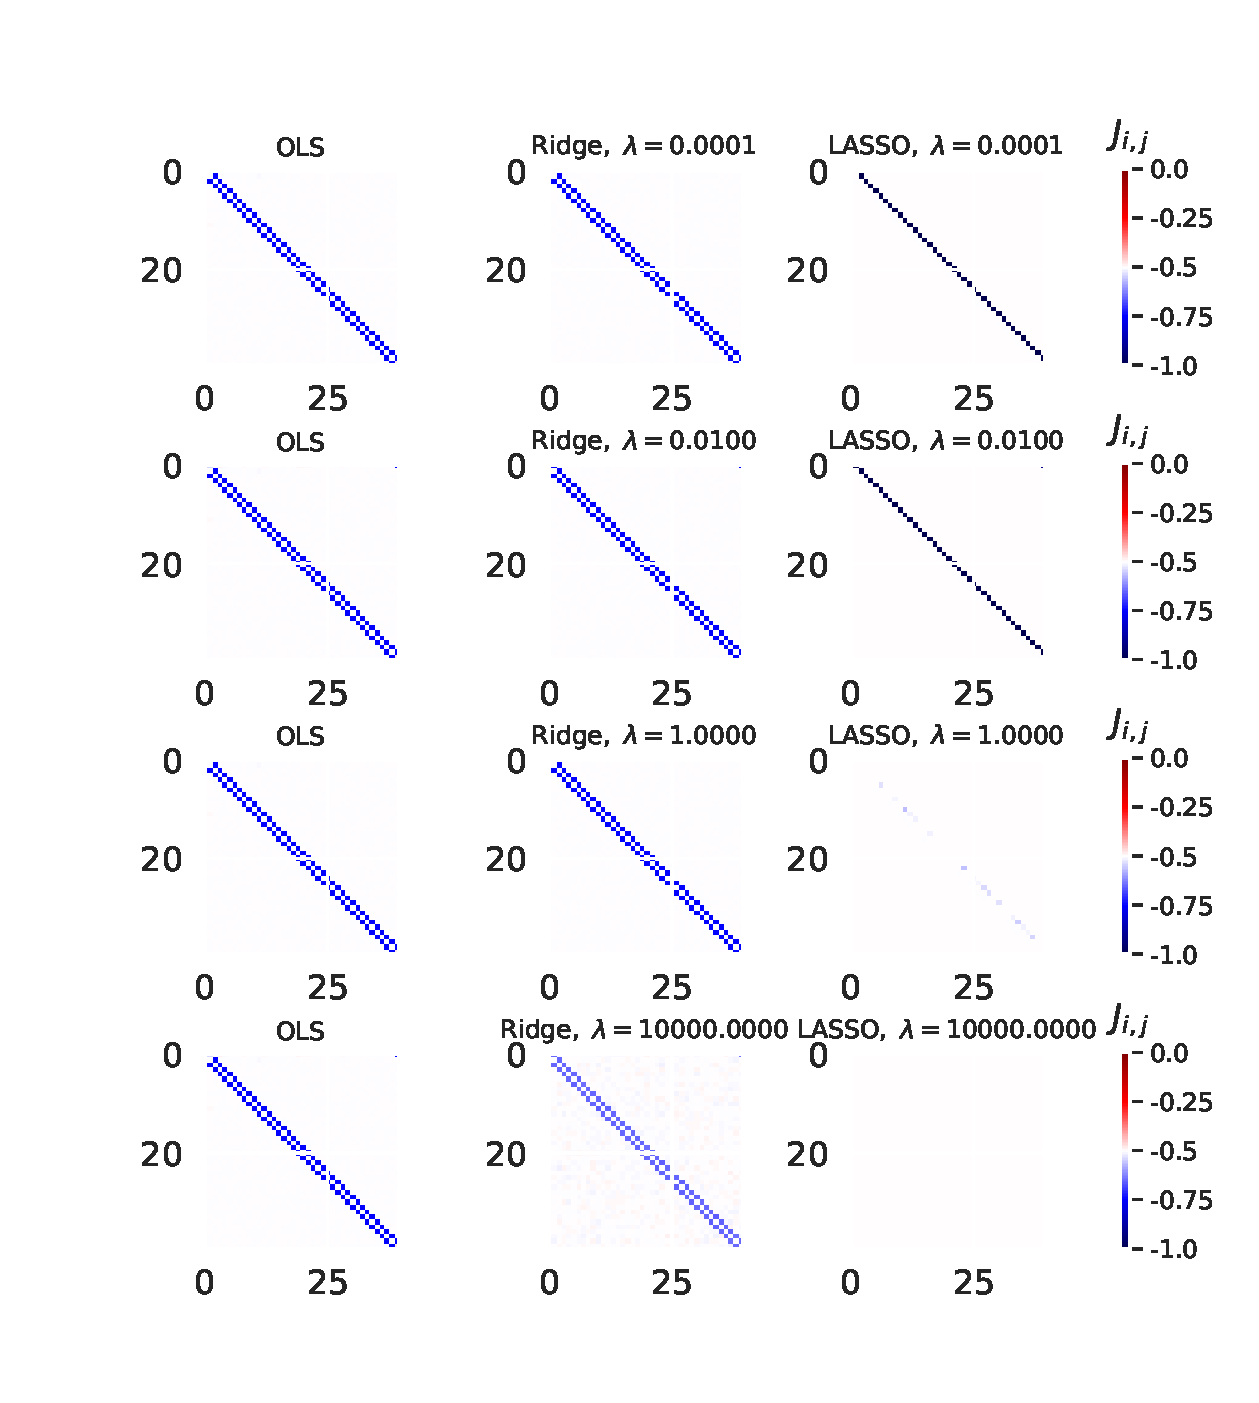
\includegraphics[width = 0.7\paperwidth]{figures/regression_mehtastyle.pdf} 
\caption{Ising model plots for selected regularization parameters $\lambda$, generated based on our regression models.
	 } 
\label{fig:regression-mehta}
\end{figure}

\begin{figure}[H]
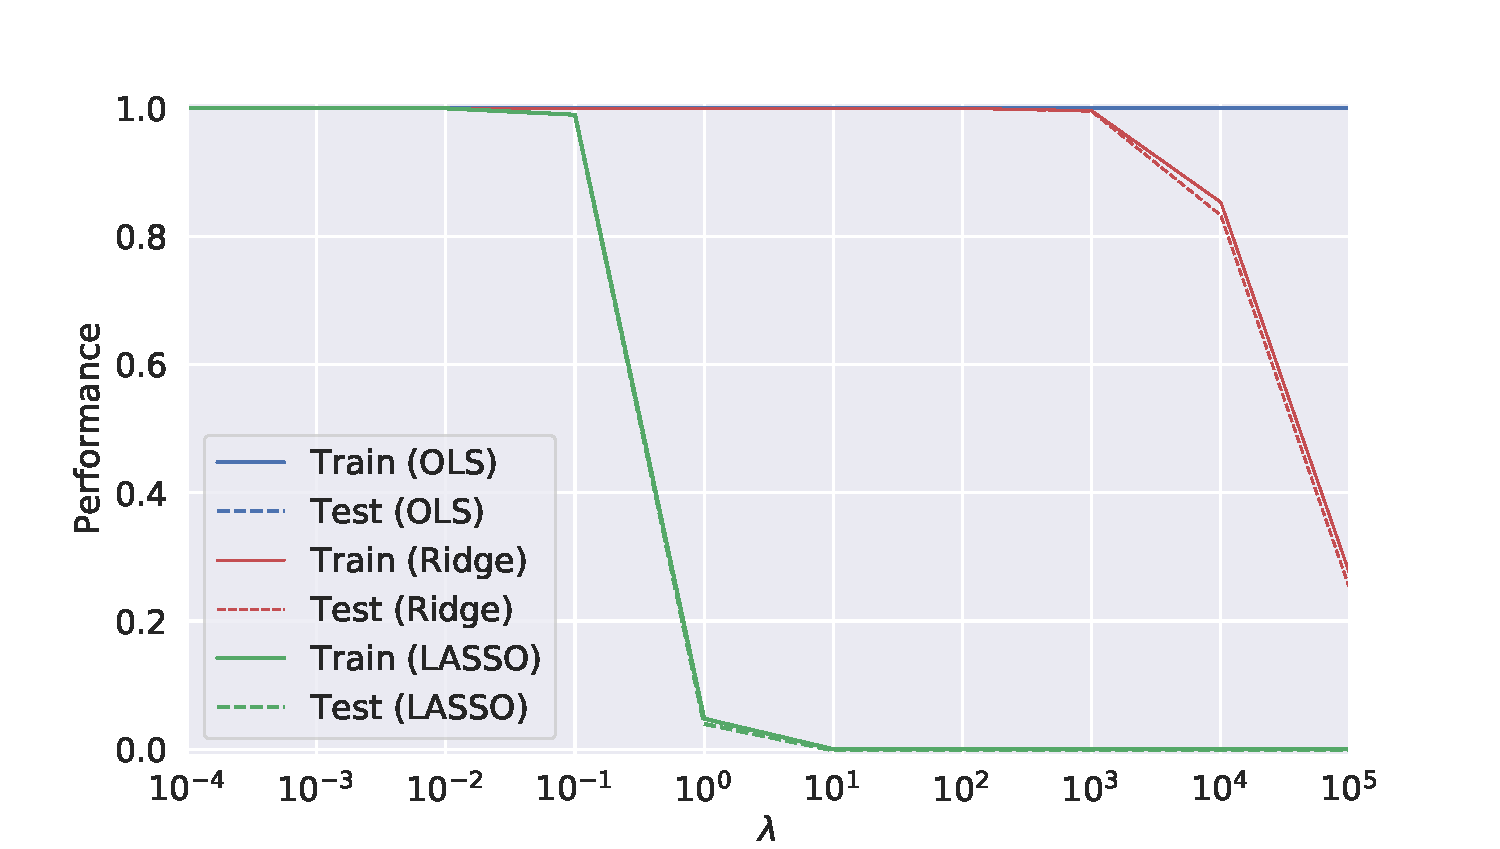
\includegraphics[width = 0.8\paperwidth]{figures/regression_r2.pdf}
    \caption{R2 score performance of the linear regression models as a function of
	     regression parameter $\lambda$.}
\label{fig:regression-r2}
\end{figure}

Figure \ref{fig:regression-r2} show how the R2 score varies between models. 
It's important to note that the $\lambda$ for Ridge regression, and $\alpha$ 
for Lasso regression have the same value, but they affect the models on 
different orders of magnitude, and must be treated somewhat separately. 
Even so, we can see that the training and test set R2-scores
follow eachother closely.

Figure \ref{fig:regression-r2-article} is from article ~\cite{HighBias} and 
shows performance of OLS, Ridge and LASSO regression
on the Ising model as measured by the R2 coefficient of determination

\begin{figure}[H]
    \centering
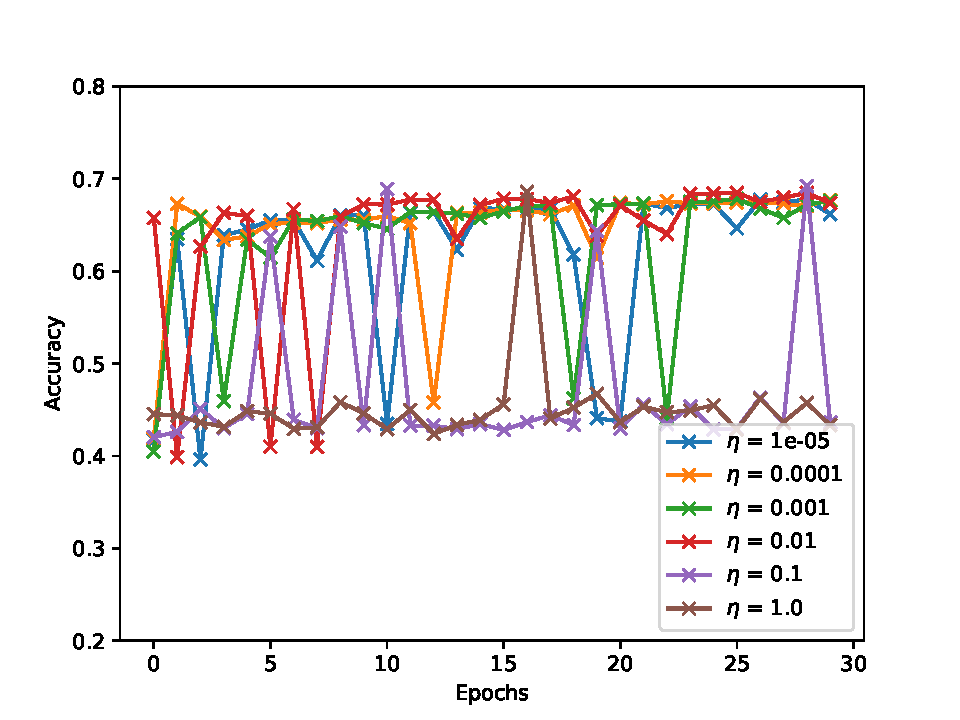
\includegraphics[width = 0.8\textwidth]{figures/logistic_eta.pdf}
    \caption{Accuracies for a selection of learning rates $\eta$ as a function of epochs. 
    30 epochs, batch size $= 100$, and momentum parameter $\gamma = 0.01$. The accuracy
    values are measured on the test set.
    The ratio of amount of training data to test data is $0.8$.}
\label{fig:logistic-eta}
\end{figure}

\begin{table}[H]
\center
\begin{tabular}{l|c|c|c}
$\eta$ & Training & Test & Critical  \\
\hline
$10^{-5}$ & $0.718$ & $0.680$ & $0.616$ \\
$10^{-4}$ & $0.723$ & $0.683$ & $0.624$ \\
$10^{-3}$ & $0.723$ & $0.685$ & $0.628$ \\
$10^{-2}$ & $0.712$ & $0.672$ & $0.604$ \\
$10^{-1}$ & $0.462$ & $0.430$ & $0.460$ \\
$1$    & $0.465$ & $0.446$ & $0.480$
\end{tabular}
    \caption{Accuracies for a selection of learning rates $\eta$ after 
    30 epochs. Batch size $= 100$, and momentum parameter $\gamma = 0.01$.
    The ratio of amount of training data to test data is $0.8$}
    \label{tab:logistic-critical}
\end{table}
In table \ref{tab:logistic-critical} the accuracy on data containing critical 
states is included. Due to the varying nature our logistic model, a solution 
in which the weights producing the best fit on test data are stored was 
developed. The accuracies for the critical states are thus not necessarily 
produced with weights as they are after 30 epochs. The reason for this 
descrepancy is yet to be found.

\subsection{Classifying with Neural Network}
\begin{figure}[h]
    \centering
    \subfloat[]{
	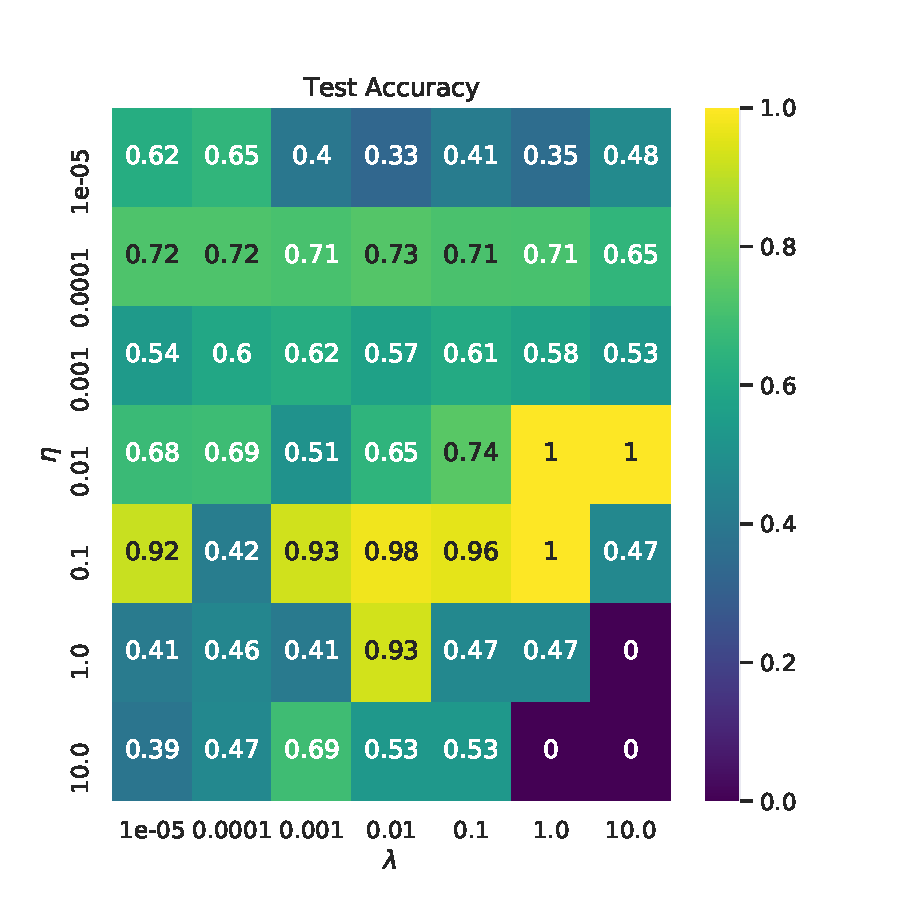
\includegraphics[width=0.55\textwidth]{figures/net_acc_test_1.pdf}
	}
    \subfloat[]{
	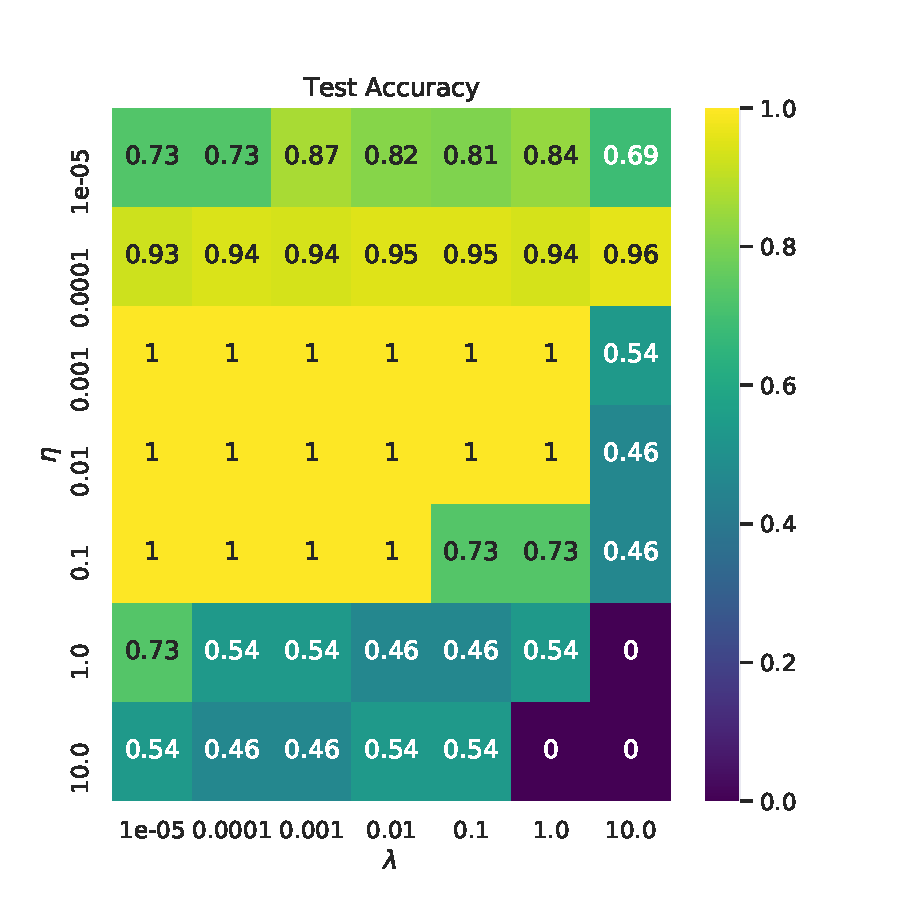
\includegraphics[width=0.55\textwidth]{figures/net_acc_test_2.pdf}
	}\\
    \subfloat[]{
	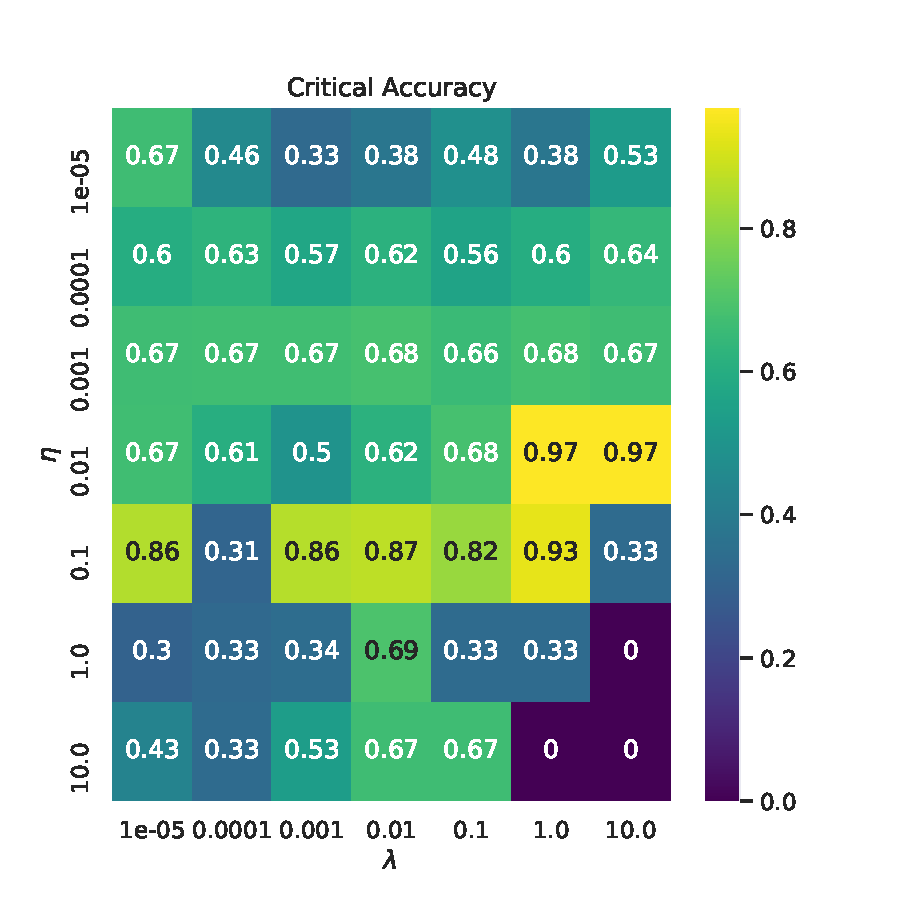
\includegraphics[width=0.55\textwidth]{figures/net_acc_crit_1.pdf}
	}
    \subfloat[]{
	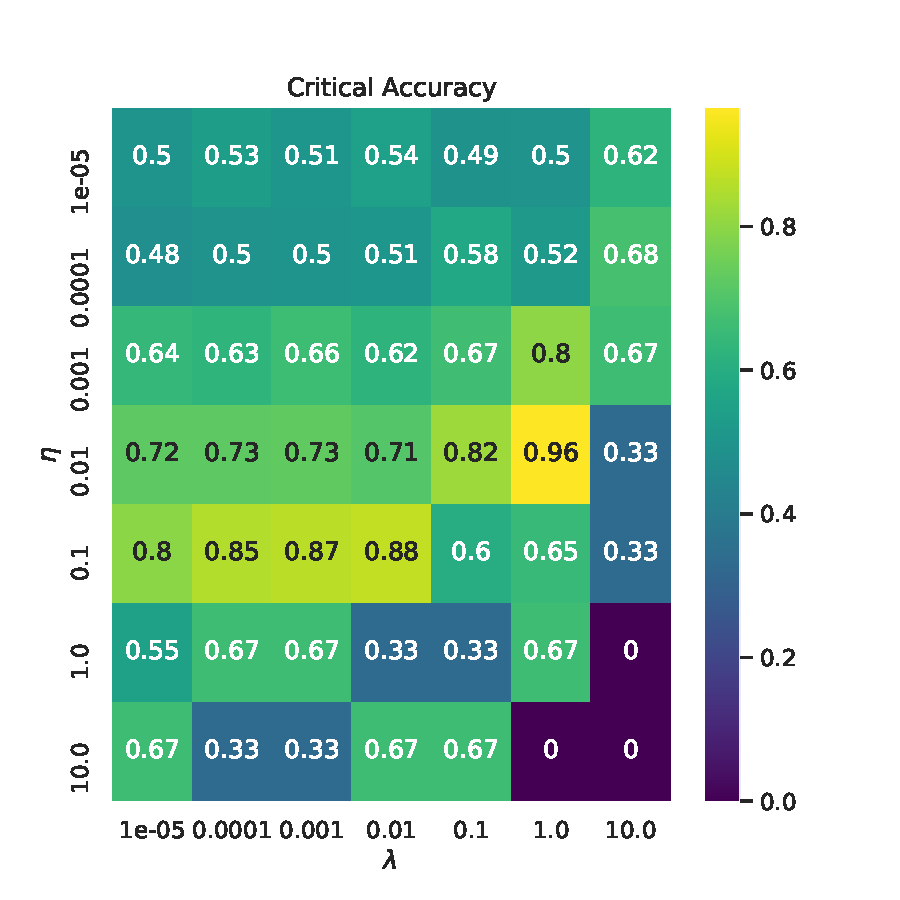
\includegraphics[width=0.55\textwidth]{figures/net_acc_crit_2.pdf}
	}
    \caption{
	Neural network classification accuracies for grid search across 
	learning rates $\eta$ and regularization parameters $\lambda$ on 
	the test and critical set after 10 epochs.
	a),c) show the network with one hidden layer, 10 nodes. 
	b), d) show the network with two hidden layers of size 100 (first) and 50
	(second). 
	}
    \label{fig:nn-grids}
\end{figure}
Grid search across multiple orders of magnitude of learning rate and
regularization parameter is shown in figure \ref{fig:nn-grids}. 
Both network architectures were trained on 
$10\%$ of the available samples from the ordered and disordered states.
Comparing the values with those presented in table \ref{tab:logistic-critical},
the network performs much better in classifying the states.
The grid search shows that for the test set the larger architecture with two layers
perform very well on the test set across multiple combinations of parameters,
while the single-layer is more sensitive to the parameter choice.
The performance on the test set is, however, not reflected in the two architectures'
performance on the data from the critial temperature region, as seen in figure 
\ref{fig:nn-grids} (c,d), where the single-layer network actually outperforms the
multilayer network slightly.

\section{Discussion}
Based on figures \ref{fig:regression-mehta} and 
\ref{fig:regression-mehta-article}, we see that the figure in article 
~\cite{HighBias} is similar to our own figures. 
Compared to the plots in the article our plots shows less noice, 
and some other small differences, but we see that the tendencies are the same.

Looking at the R2 scores from figure \ref{fig:regression-r2}, we see 
that the R2 score for the training and test set follow each other closely. 
Again, comparing with articles plot, shown in figure 
\ref{fig:regression-r2-article}, we see the two have a similar shape 
but that there are a bigger diggerence between the R2 score for training 
data and the test data in the article. 
In the articles figure, the difference seems to be biggest for Ridge and 
OLS. As for our plot, it seems like Ridge has a bit bigger difference 
between the R2 score for training and test data than for the two other 
methods. 



\section{Conclusion}
In this work four methods to sample or manipulate input data to learning
algorithms are explored: Random over-sampling, SMOTE, ADASYN, and balanced
weighting.
Using Cumulative Gain Charts, Confusion Matrices and
ROC curves, and cross-validation, the performance of a logistic regression 
algorithm, and a random forest classifier is evaluated based on how they 
perform on a binary classification problem. 
The data set chosen is payment data from an important bank in Taiwan,
where the data describes credit card holders, and the goal is predicting
whether a customer will default the next payment or not. This allowed for
comparisons with \cite{ComparisonData}. The results presented show that
logistic regression can classify the credit card data perfectly by applying
a balanced weighting of the inputs. Random forests reached an accuracy of
~$95\%$ (cross-validation score). A possible explanation for the success of
weighting the inputs compared to the other sampling methods is presented. 
Specifically, some features in the data set may be far more crucial in
determining the class than others, and weighting is the most efficient way of
emphasizing these features through the learning process.
This works only for the logistic model, however. For random forests, the
most improvement was found when using random over-sampling.

For future studies, an in-depth look at which features are the most important,
and how the different models evaluate this, could be very interesting, as it
may reveal some underlying effects of the sampling techniques.


\appendix
\bibliographystyle{unsrt}
\bibliography{bibliography}
\end{document}
